\chapter{Cahier des charges}

\section{Budget}

Ce projet s'inscrit dans le cadre de l'UV S28, il n'y a donc pas de budget. Néanmoins, une \textbf{lourde charge de travail} est à prévoir, dûe à la découverte de Unity.

\section{Ressources médias}

Notre jeu n'utilise pas de ressource particulière de type image ou vidéo. Il s'agit uniquement d'un environnement 3D virtuel, composé de formes géométriques (les murs du labyrinthe) générées grâce au code informatique.

\medskip

En revanche, il utilisera cependant une musique de fond, \og stressante\fg{}. Cela a pour but d'\textbf{accroître l'immersion et d'accentuer l'ambiance oppressante d'un labyrinthe.}. De plus, des sons plutôt effrayants permettent de jouer sur les émotions.

\medskip

Enfin, quelques textes sont affichés à différents moments du jeu à l'utilisateur (voir chapitre \ref{scenario} du rapport ci-contre).

\medskip

D'autres éléments textuels sont susceptibles d'être ajoutés, en fonction du développement d'autres fonctionnalités (cela dépendra du temps que nous avons, cf \ref{sub:objectifs_complementaires}).

\bigskip

Ce jeu est \textbf{dynamique} : l'utilisateur est dans un environnement sur lequel il ne peut agir mais dans lequel il peut se déplacer de façon naturelle (ce n'est pas une succession d'images, ni une vidéo). Les mouvements réels du joueurs sont retransmis de manière presque naturelle dans le jeu. \textbf{La vue est à la première personne} : le joueur ne peut se voir.

\section{Structure et navigation}

Le jeu contiendra un seul type de contenu : le jeu. Il n'y a pas de menu puisqu'aucun réglage n'est proposé à l'utilisateur (pas de paramètre de jeu).

\subsection{Le jeu}
Dès le lancement de l'application sur son téléphone, le jeu démarre. Un texte apparaît : \og{}Trouvez la sortie\fg{}.

\medskip

Si le joueur désire quitter le jeu, il doit utiliser le bouton \og Retour\fg{} de son téléphone. L'écran d'accueil du téléphone apparaît alors.

\medskip

Il n'y a pas d'autre forme de navigation dans le jeu : le joueur se déplace uniquement dans un environnement virtuel 3D, comme dans un jeu vidéo, en essayant de trouver la sortie du labyrinthe dans lequel il se trouve.

\section{Formes et degrés d'interactivité}

L'interactivé réside dans l'immersion du joueur dans son environmment virtuel qu'est le labyrinthe. Il ne peut pas interagir avec en le modifiant par exemple, seulement s'y déplacer. Du vent fait mouvoir des objets (un arbre par exemple) dans le jeu, de manière à le rendre plus vivant.

\section{Choix techniques}

Notre jeu est développé pour la plateforme \textbf{Android}. Nous n'avons pas utilisé OpenGL puisque cette technologie nous était inconnue et bien trop longue à appréhender. C'est la raison pour laquelle nous nous sommes tournés vers \textbf{Unity}, qui est un moteur graphique beaucoup plus rapide à prendre en main (notamment grâce à de nombreux outils graphiques).

\medskip

Nous utilisons donc les outils fournis par Unity pour générer notre environnement 3D. Le jeu est ainsi développé dans le logiciel Unity.

\begin{figure}[h!]
  \centering
  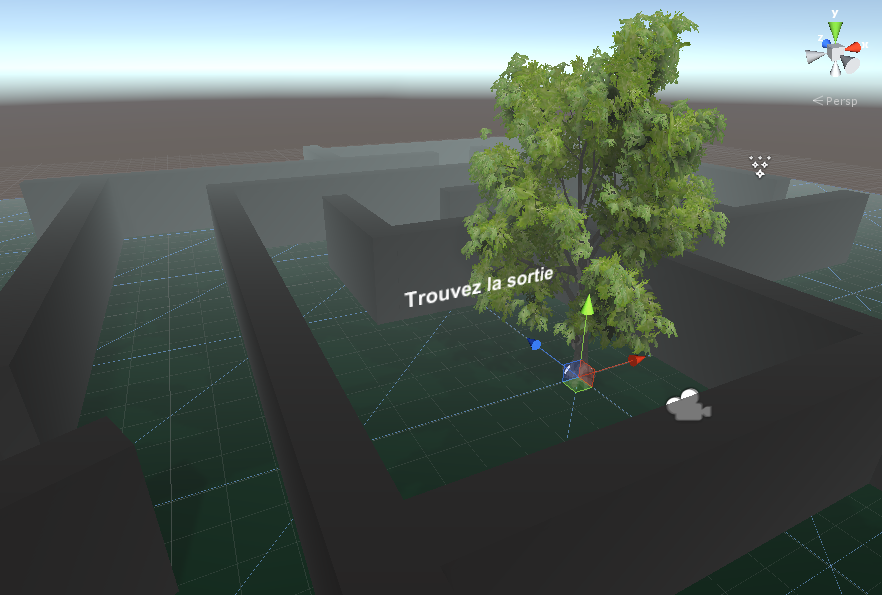
\includegraphics[width=1.0\textwidth]{res/img/unity.png}
  \caption{Création du labyrinthe sous Unity}
\end{figure}